\documentclass[13pt]{article}
\usepackage{amsmath}
\usepackage{amsfonts}
\usepackage{amssymb}
\usepackage{kotex}
\usepackage[export]{adjustbox}
\usepackage{mathtools}
\usepackage{graphicx}
\usepackage{wrapfig}
\graphicspath{ {images/} }
\usepackage{geometry}
	\geometry{
		top = 20mm,
		left = 20mm,
		right = 20mm,
		bottom = 20mm,
		}
\geometry{a4paper}
		
\pagenumbering{gobble}
\renewcommand{\baselinestretch}{1.3}

\begin{document}
\begin{center}
\textbf{\Large 전기전자회로 Chapter 3 Problem Solving} \\
\large 2017-18570 컴퓨터공학부 이성찬
\end{center}

\subsubsection*{Example 2.28} 
\begin{wrapfigure}{r}{0.3\textwidth}\centering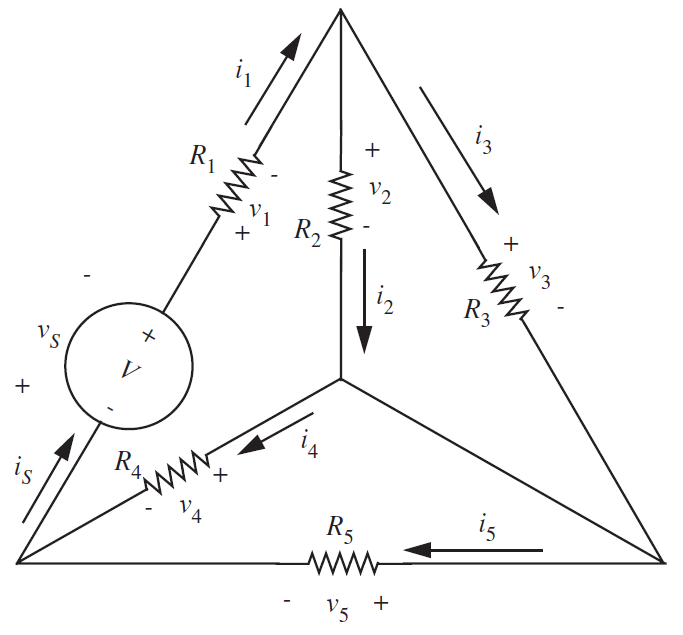
\includegraphics[width=0.3\textwidth]{ex2_28}\end{wrapfigure}
다음과 같이 변수들과 방향을 설정한다. 그러면 $$v_s=-V, \quad v_n=R_ni_n \quad \text{for } n = 1, \dots, 5$$ 이고 KVL 으로부터
\begin{align}
-V+i_1R_1 + i_2R_2 + i_4R_4 = 0
\end{align}
그리고 옴의 법칙을 활용하면 $$i_2 = i_1\frac{R_3}{R_2+R_3}, \quad i_4 = i_1\frac{R_5}{R_4+R_5}$$
이를 (1)에 대입하면 $i_S=i_1$ 이므로
$$V = i_1R_1 + i_2R_2 + i_4R_4 = i_S\left(R_1 + \frac{R_2R_3}{R_2+R_3} + \frac{R_4R_5}{R_4+R_5}\right)$$

\subsubsection*{Exercise 3.15}
\begin{wrapfigure}{r}{0.35\textwidth}
	\centering
	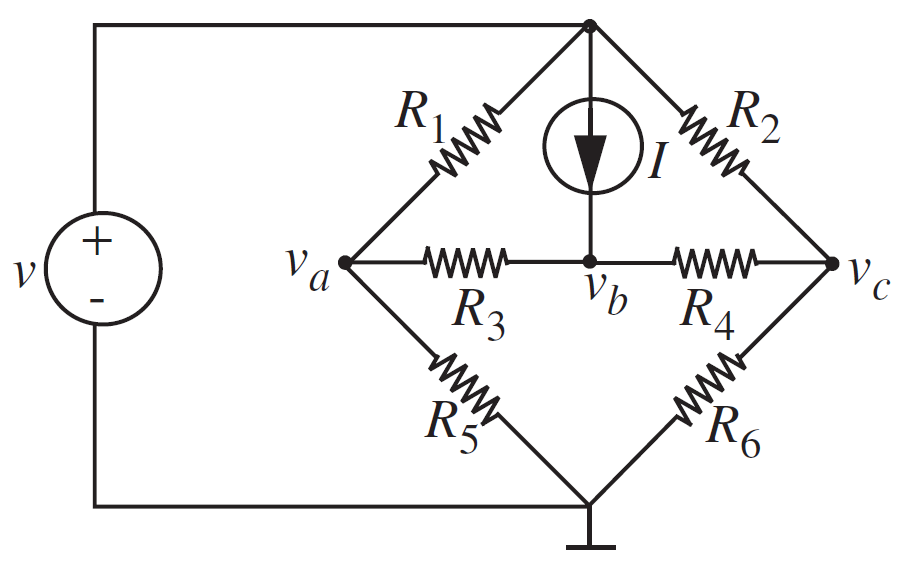
\includegraphics[width=0.35\textwidth]{ex3_15}
\end{wrapfigure}
저항 $R_n$ 이 존재하는 branch 에 흐르는 전류를 $i_n$ 이라고 하자.\\ $n = 1, 2, 5, 6$ 의 경우 전류는 위에서 아래로 흐르고, $n = 3, 4$ 의 경우는 오른쪽에서 왼쪽으로 흐른다고 가정한다. 또한 맨위 지점과 맨 아래 접지된 지점의 node voltage 는 각각 $v, 0$ 이다. \\ 이제 KCL 을 node voltage 가 $v_a, v_b, v_c$ 인 지점에 각각 적용하면,
\begin{align*}
i_4&=I+i_3 \\ i_1&=i_3+i_5 \\ i_6 &= i_2+i_4
\end{align*}
이므로 이에 대응하는 branch current 를 Ohm's Law 로 계산하여 대입하고 conductance $G_n = 1/R_n$ 으로 정의한다. 그러면
\begin{align*}
G_4(v_b-v_c) &= I + G_3(v_a-v_b) \\ 
G_1(v-v_a) &= G_3(v_a-v_b) + G_5(v_a - 0) \\ 
G_6(v_c - 0) &= G_2(v - v_c) + G_4(v_b-v_c)
\end{align*}
를 얻을 수 있고, 정리하면
\begin{align*}
(G_1+G_3+G_5)v_a - G_3v_b + 0\cdot v_c &= G_1v \\
0\cdot v_a - G_4v_b + (G_2+G_4+G_6)v_c &= G_2v\\
G_3v_a - (G_3+G_4)v_b + G_4v_c &= -I
\end{align*}

\pagebreak

\subsubsection*{Exercise 3.25}
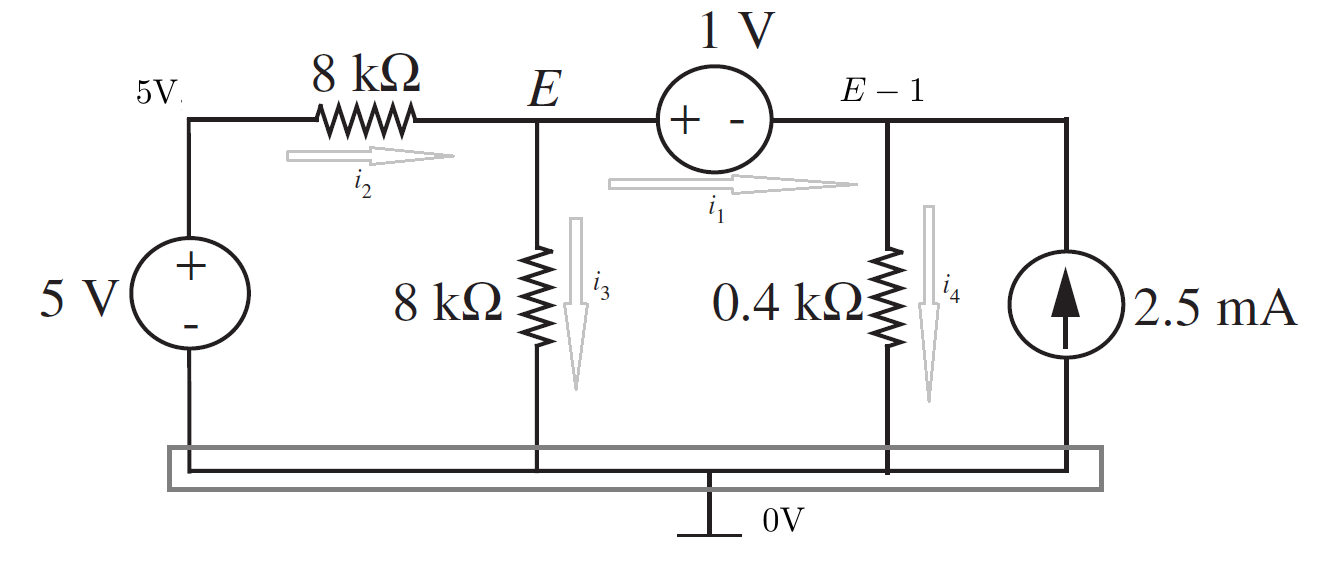
\includegraphics[width=0.7\textwidth, center]{ex3_25}\\
위와 같이 설정하면, node voltage 가 $E, E-1$ 인 지점에서 각각 KCL 을 적용하여 $$i_2 = i_1+i_3, \quad i_4 = i_1 + 2.5$$ 를 얻는다. Branch current 를 계산하여 대입하면
$$\frac{5-E}{8} = \frac{E - 0}{8} + i_1, \quad i_1+2.5 = \frac{E-1}{0.4}$$ 를 얻고 $i_1$ 을 소거하면 $\boxed{E=45/22\:(\text{V})}$ 를 얻는다.

\subsubsection*{Problem 3.8}
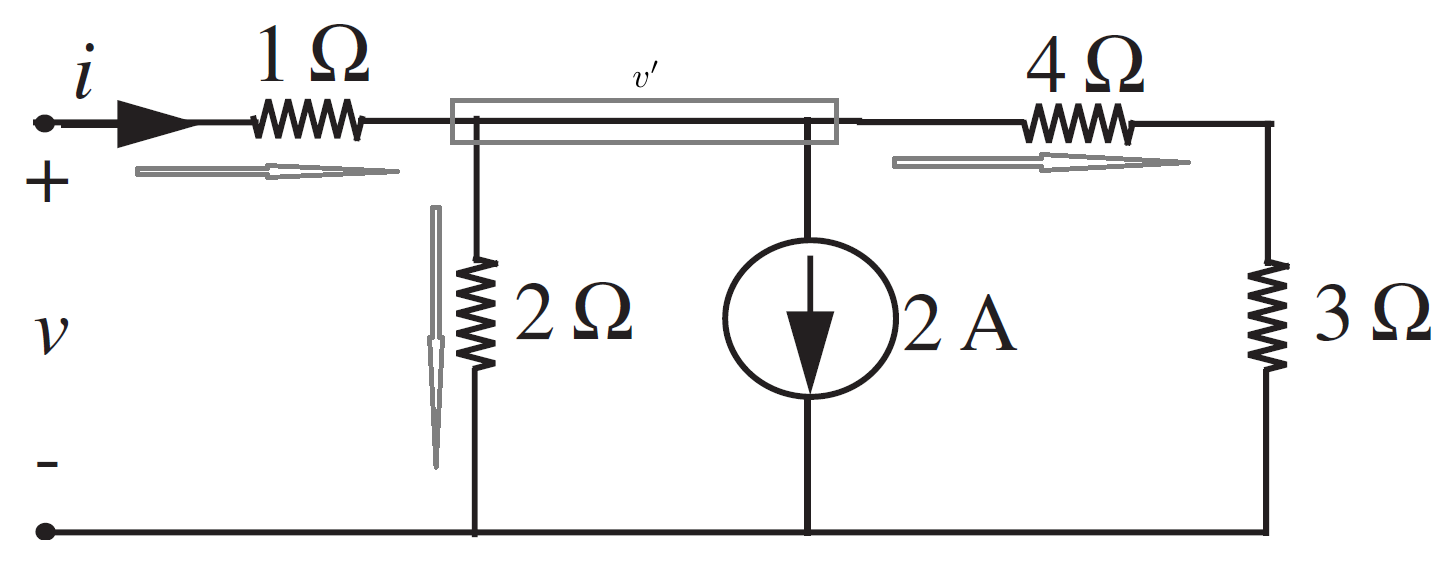
\includegraphics[width=0.5\textwidth, center]{p3_8}
\begin{itemize}
\item[(a)] 위와 같이 전류가 흐른다고 가정하면 node voltage 가 $v'$ 인 지점에서 KCL 에 의해 $$\frac{v-v'}{1} = \frac{v'-0}{2} + 2 + \frac{v'-0}{7} \qquad \therefore v'=\frac{14v-28}{23}$$
그리고 $i = (v-v')/1$ 이므로 대입하여 정리하면 $\displaystyle \boxed{v = \frac{23}{9}i - \frac{28}{9}}$

\item[(b)] 그래프를 그리면 된다.\\
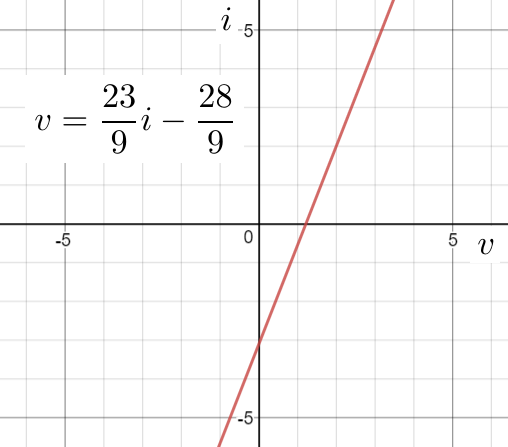
\includegraphics[width=0.4\textwidth, center]{p3_8b}
\item[(c), (d)] Use the relation $v = v_{TH} + R_{TH}i$, $i_N = v_{TH} / R_{TH}$ and the answer from (a).\\
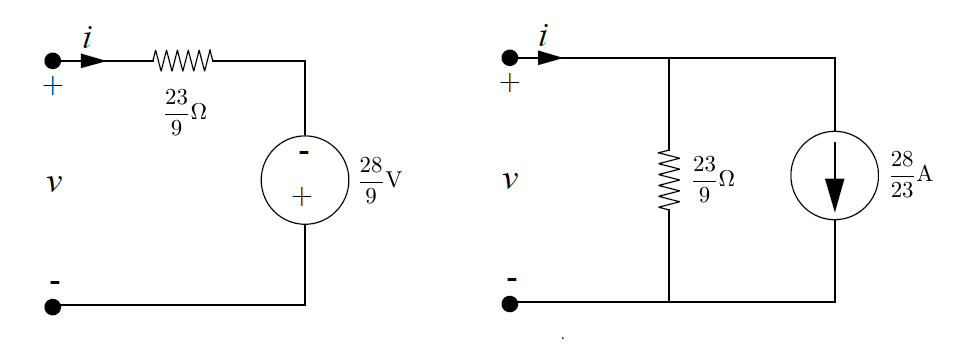
\includegraphics[width=0.8\textwidth, center]{p3_8cd}
\end{itemize}

\subsubsection*{Problem 3.9}
\begin{itemize}
\item[(a)] The current acting alone, then the voltage is $$8 \times \frac{6/7 \cdot 6}{6 + 6/7}\times \frac{4}{6} = -4\mathrm{V}$$
The voltage source acting alone, then the voltage is $$A_0\times \frac{3}{4}\times \frac{4}{6} = \frac{A_0}{2} \mathrm{V}$$
By superposition, $\boxed{v_0 = A_0/2 - 4 \:(\mathrm{V})}$
\item[(b)] Define node voltages and branch currents as follows. \\
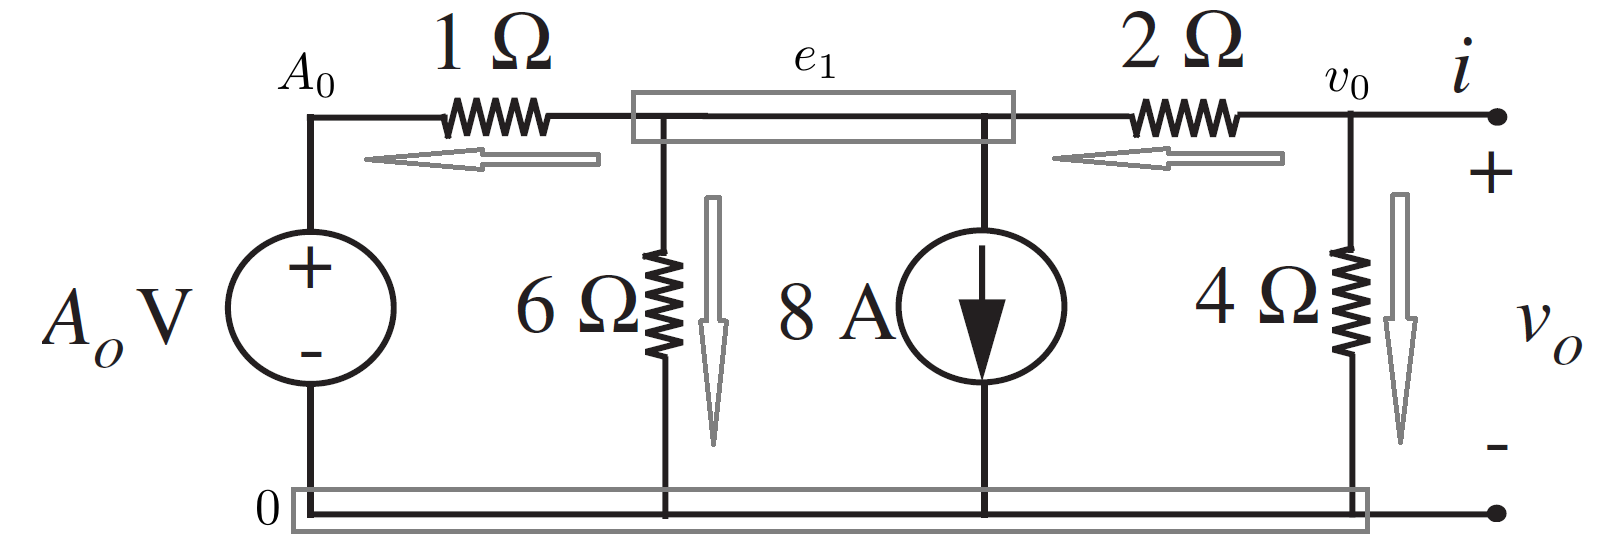
\includegraphics[width=0.5\textwidth, center]{p3_9}\\
Then by applying KCL at the nodes with node voltage $e_1$ and $v_0$, $$\frac{e_1-A_0}{1}+\frac{e_1 - 0}{6} + 8 = \frac{v_0-e_1}{2}, \quad \frac{v_0-0}{4} + \frac{v_0-e_1}{2} = 0$$
Solve for $v_0$ to get the final result, $\boxed{v_0 = A_0/2 - 4 \:(\mathrm{V})}$
\end{itemize}








\end{document}
